% !TeX spellcheck = en_US
\section{Empirical Study Design}\label{sec:design}
\IEEEPARstart{T}{he} \textit{goal} of the study is to perform an historical analysis of the test-suites related to components affected by \asmells in open-source systems, with the \textit{purpose} of assessing whether the quality of these test suites decreases when \asmells are introduced.
Moreover, the study aims to asses how the fault proneness of the considered components varies when these smells occur.


\subsection{Context selection}
The context of our study is made up of \asmells and software systems.
Among the currently known \asmells, we considered the following package level Architectural Smells: %[LISTA DI SMELLS].
\begin{itemize}
  \item \textbf{God Component:} the component contains a high number of classes.
  \item \textbf{Cyclic Dependency:} this component participates in a cyclic dependency. 
  \item \textbf{Unstable Dependency:} this component depends on other components that are less stable than itself.
  \item \textbf{Feature Concentration:} the component realizes more than one architectural concern/feature. 
  \item \textbf{Dense Structure:} all the analyzed components exhibit excessive and dense dependencies among themselves. 
  \item \textbf{Ambiguous Interface:} the component provides only a single general entry-point via a class.
\end{itemize}

Moreover, \cyclic and \hublike are well-known smells and object of a great number of studies \cite{IEEEhowto:systematicmapping}. 
However, for the opposite reason, we chose to focus on class level Architectural Smells, since, as explained by \cite{IEEEhowto:systematicmapping}, they have never been studied, and so we focused on:
\begin{itemize}
  \item \textbf{Deficient Encapsulation:} This smell occurs when the declared accessibility of one or more members of abstraction is more permissive than required.
  \item \textbf{Unutilized Abstraction:} This smell arises when an abstraction is left unused (either not directly used or not reachable).
  \item \textbf{Feature Envy:} This smell occurs when a method seems more interested in a class other than the one it is in.
  \item \textbf{Broken Hierarchy:} This smell arises when a super-type and its sub-type conceptually do not share an "IS-A" relationship resulting in broken substitutability.
  \item \textbf{Broken Modularization:} This smell arises when data and/or methods that ideally should have been localized into a single abstraction are separated and spread across multiple abstractions.
  \item \textbf{Insufficient Modularization:} This smell arises when an abstraction exists that has not been completely decomposed, and a further decomposition could reduce its size, implementation complexity, or both.
  \item \textbf{Wide Hierarchy:} This smell arises when an inheritance hierarchy is "too" wide indicating that intermediate types may be missing.
  \item \textbf{Unnecessary Abstraction:} This smell occurs when an abstraction that is not needed (and thus could have been avoided) gets introduced in a software design.
  \item \textbf{Multifaceted Abstraction:} This smell arises when an abstraction has more than one responsibility assigned to it.
  \item \textbf{Cyclically-dependent Modularization:} This smell arises when two or more abstractions depend on each other directly or indirectly.
  \item \textbf{Cyclic Hierarchy:} This smell arises when a super-type in a hierarchy depends on any of its sub-types.
  \item \textbf{Rebellious Hierarchy:} This smell arises when a sub-type rejects the methods provided by its super-type(s).
\end{itemize}
We chose these because they all occur at the class level, so we could conduct our study at the same level of granularity.
To compute these Architectural Smells we have chosen to use a tool called Designite \cite{IEEEhowto:designite}, which allows the computation of all the smells previously described for the Java projects.\par\hfill

Regarding Test Smells we focused on static analysis to detect these and in particular we considered the following:
\begin{itemize}
  \item \textbf{It1 (Ignored Test):} A test method or class that contains the \verb|@Ignore| annotation.
  \item \textbf{Gf1 (General Fixture):} Not all fields instantiated within the \verb|setUp()| method of a test class are utilized by all test methods in the same test class.
  \item \textbf{Ro1 (Resource Optimism):} A test method utilizes an instance of a \verb|File| class without calling the \verb|exists()|, \verb|isFile()| or \verb|notExists()| methods of the object.
  \item \textbf{Ar1 (Assertion Roulette):} A test method contains more than one assertion statement without an explanation/message (parameter in the assertion method).
  \item \textbf{Et1 (Eager Test):} A test method contains multiple calls to multiple production methods.
  \item \textbf{Mg1 (Mystery Guest):} A test method containing object instances of files and databases classes.
  \item \textbf{Se1 (Sensitive Equality):} A test method invokes the \verb|toString()| method of an object.
\end{itemize}

\subsection{Data analysis}
For the computation of these metrics has been chosen the tool VITRuM \cite{{IEEEhowto:vitrum}}, this tool was only a tool for IntelliJ Plugin, but it was adapted to be used by Command Line Interface too, and for this reason, we used this tool for static analysis of test cases.\par\hfill

The first step was the selection of GitHub projects and to chose what project mine we used these criteria:
\begin{itemize}
  \item Only Java project.
  \item Minimum release number: 10.
  \item Minimum star number: 10.000.
  \item Exclude fork.
\end{itemize}

With these criteria, we selected 90 projects, and on these projects, we used the framework RepoDriller that allows the mining of the repository \cite{{IEEEhowto:repodriller}}. Using this framework we mined all these repository releases and for every release, we launched Designite, to detect Architectural Smells, and VITRuM, to detect Test Smells, to collect the information about all these smells. All the results returned for every release were merged in a unique CSV file with some additional columns, in particular, the columns are: 
\begin{itemize}
  \item \textbf{HashTag:} the name of the current release.
  \item \textbf{HashCommit:} the hash of the corresponding commit.
  \item \textbf{Date:} the date of the commit.
\end{itemize}
We added these three columns for both Architectural Smells and Test Smells CSV files.

\begin{figure}[htp]
    \centering
    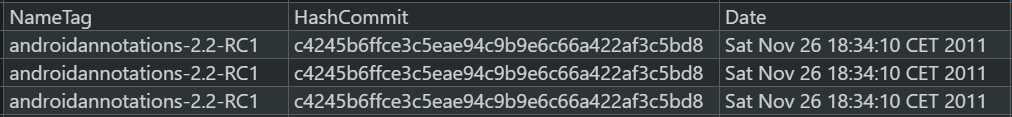
\includegraphics[width=8cm]{img/colonneAggiunte.PNG}
    \caption{Example of the three added column}
    \label{fig:rowAdditional}
\end{figure}

Unfortunately, during the mining, there were some problems with the computation of Designite for some projects, because it could not detect smells and for this reason, they were put aside. There were some problems with VITRuM too and in particular, we couldn't analyze some projects because they didn't have test cases and so there was nothing to analyze or some projects didn't have the correct structure \verb|src/test| that VITRuM finds with the aim of analyzing the projects. The problem of the structure was present when the project was organized in modules, and to resolve this we created a recursive function that analyzed these modules and runs VITRuM on single modules, after that the results were merged all in one. In some other cases, some projects did not have the test folder called \verb|test|, for example, they had \verb|testRun| or similar, and so VITRuM couldn't find it and consequently couldn't analyze the test cases of these projects.
For these reasons, the number of projects passed from 90 to 40, but fortunately, it was not a small number, especially because we selected only big projects with a minimum of 10 releases, and it allowed us to conduct the analysis of the resultant data.
